\chapter{अभिक्रियाओं की ऊर्जा: दहन और आबंध ऊर्जाएँ}\label{ch:g11:reaction-energy}

हाथ गरम करने वाली थैली की सील तोड़िए और एक मिनट बाद वह इतनी गरम हो जाती है कि
देर तक पकड़ी नहीं जा सकती; एक शीत पैक को दबाइए और वह मोच खाए टखने को ठंडक देता है; शहर की एक
बस दिन भर हाइड्रोजन पर चलती है और अपने पीछे केवल जलवाष्प छोड़ती है।
रासायनिक रूपांतरण केवल पदार्थों को दूसरे पदार्थों में ही नहीं बदलते: वे
ऊर्जा मुक्त करते हैं, या ग्रहण करते हैं। वह ऊर्जा कहाँ से आती है, और
कोई \omterm{def:g4:what-a-fire-needs:fuel}{ईंधन} उसकी कितनी मात्रा दे सकता है?

\begin{recall}
\omterm{def:g8:combustion-and-fuels:complete}{पूर्ण दहन} में कार्बन और हाइड्रोजन से बना \omterm{def:g4:what-a-fire-needs:fuel}{ईंधन}
डाइऑक्सीजन में जलकर कार्बन डाइऑक्साइड और पानी देता है
(\cref{ch:g8:combustion-and-fuels})। \omterm{def:g10:lewis-and-shape:covalent-bond}{सहसंयोजी आबंध} \omterm{def:g9:inside-the-atom:nucleus}{इलेक्ट्रॉनों} का एक साझा
युग्म है; \omterm{def:g10:lewis-and-shape:lewis-structure}{लुइस संरचनाएँ} किसी \omterm{def:g7:atoms-and-molecules:molecule}{अणु} का हर आबंध दिखाती हैं
(\cref{ch:g10:lewis-and-shape})। \omterm{def:g10:the-mole:amount}{पदार्थ की मात्रा} \omterm{def:g10:the-mole:amount}{मोल} में गिनी जाती है
(\cref{ch:g10:the-mole})।
\end{recall}

\begin{omfigure}
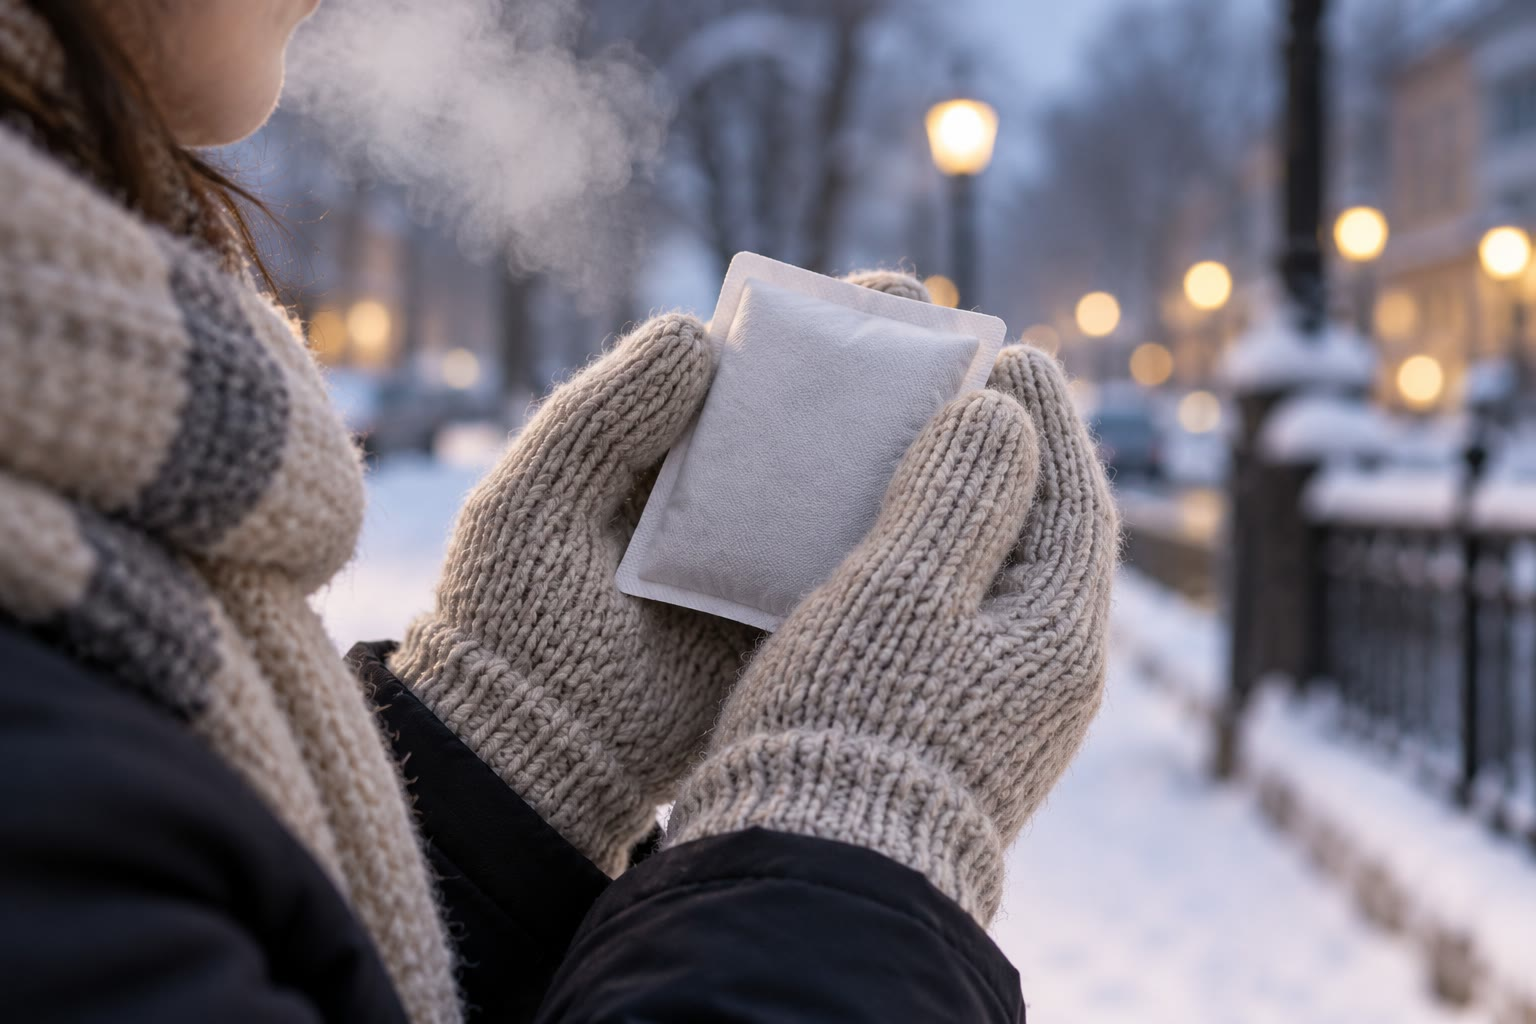
\includegraphics[width=0.45\linewidth]{images/book1/ai/g11-hand-warmers.jpg}

{\small हाथ गरम करने वाली थैली: थैली के भीतर एक अभिक्रिया ऊष्मा मुक्त करती है।}
\end{omfigure}

\section{ऊष्माक्षेपी और ऊष्माशोषी रूपांतरण}

\begin{definition}[ऊष्माक्षेपी, ऊष्माशोषी]\label{def:g11:reaction-energy:exothermic}
कोई रूपांतरण \emph{ऊष्माक्षेपी}\index{ऊष्माक्षेपी} है यदि वह अपने परिवेश को
ऊर्जा देता है, आम तौर पर ऊष्मा के रूप में: परिवेश गरम होता है।
वह \emph{ऊष्माशोषी}\index{ऊष्माशोषी} है यदि वह अपने परिवेश से ऊर्जा
ग्रहण करता है: परिवेश ठंडा होता है, या रूपांतरण को जारी रहने के लिए
गरम करना पड़ता है।
\end{definition}

\begin{example}[गरम और ठंडा]\label{ex:g11:reaction-energy:packs}
\omterm{def:g4:what-a-fire-needs:burning}{दहन} \omterm{def:g11:reaction-energy:exothermic}{ऊष्माक्षेपी} होते हैं, और हाथ गरम करने वाली थैली के भीतर लोहे के चूर्ण
की \omterm{def:g4:air-a-mixture-of-gases:air}{वायु} की डाइऑक्सीजन से धीमी अभिक्रिया भी। शीत पैकों में इस्तेमाल होने वाला
पानी में अमोनियम नाइट्रेट का \omterm{def:g2:mixing-and-dissolving:dissolve}{घुलना} \omterm{def:g11:reaction-energy:exothermic}{ऊष्माशोषी} है; वैसे ही चूना-पत्थर का
बिना बुझे चूने और कार्बन डाइऑक्साइड में अपघटन भी, जो केवल
बहुत गरम भट्ठे में होता है।
\end{example}

\begin{omfigure}
\begin{tikzpicture}[font=\small]
  \begin{scope}
    \draw[->] (0,0) -- (0,3.2) node[above] {ऊर्जा};
    \draw[very thick, omDef] (0.5,2.5) -- (2.3,2.5) node[right, text=black] {अभिकारक};
    \draw[very thick, omProp] (0.5,0.8) -- (2.3,0.8) node[right, text=black] {उत्पाद};
    \draw[->, thick, omThm] (1.4,2.45) -- (1.4,0.85);
    \node[omThm, anchor=west, align=left] at (1.5,1.65) {मुक्त\\ ऊर्जा};
    \node[anchor=north] at (1.6,-0.15) {\textbf{ऊष्माक्षेपी}};
  \end{scope}
  \begin{scope}[xshift=6cm]
    \draw[->] (0,0) -- (0,3.2) node[above] {ऊर्जा};
    \draw[very thick, omDef] (0.5,0.8) -- (2.3,0.8) node[right, text=black] {अभिकारक};
    \draw[very thick, omProp] (0.5,2.5) -- (2.3,2.5) node[right, text=black] {उत्पाद};
    \draw[->, thick, omDef] (1.4,0.85) -- (1.4,2.45);
    \node[omDef, anchor=west, align=left] at (1.5,1.65) {ग्रहण की गई\\ ऊर्जा};
    \node[anchor=north] at (1.6,-0.15) {\textbf{ऊष्माशोषी}};
  \end{scope}
\end{tikzpicture}

{\small ऊर्जा आरेख। \omterm{def:g11:reaction-energy:exothermic}{ऊष्माक्षेपी} अभिक्रिया में उत्पादों में \omterm{def:g7:chemical-reactions:reactant}{अभिकारकों} से कम
ऊर्जा होती है, और अंतर मुक्त होता है; \omterm{def:g11:reaction-energy:exothermic}{ऊष्माशोषी}
अभिक्रिया में उनमें अधिक होती है, और अंतर देना पड़ता है।}
\end{omfigure}

\section{दहन द्वारा मुक्त ऊर्जा}

\begin{definition}[मोलर दहन ऊर्जा]\label{def:g11:reaction-energy:combustion-energy}
किसी \omterm{def:g4:what-a-fire-needs:fuel}{ईंधन} की \emph{मोलर दहन ऊर्जा}\index{मोलर दहन ऊर्जा}
$E_c$ उसके एक \omterm{def:g10:the-mole:amount}{मोल} के \omterm{def:g8:combustion-and-fuels:complete}{पूर्ण दहन} द्वारा मुक्त ऊर्जा है,
\si{kJ/mol} में, बनने वाला पानी द्रव मानकर।
\end{definition}

\begin{proposition}[$n$ मोल द्वारा मुक्त ऊर्जा]\label{prop:g11:reaction-energy:n-moles}
% ledger: dch:CH4
\omterm{def:g4:what-a-fire-needs:fuel}{ईंधन} की मात्रा $n$ का \omterm{def:g8:combustion-and-fuels:complete}{पूर्ण दहन} ऊर्जा
$Q = n \times E_c$ मुक्त करता है। मेथेन के लिए $E_c = \qty{890.7}{kJ/mol}$: उसका
\qty{1.00}{mol} (\qty{16.0}{g}) \omterm{def:g4:what-a-fire-needs:burning}{जलाने} पर लगभग \qty{891}{kJ} मुक्त होती है।
\end{proposition}

\begin{proof}
\omterm{def:g4:what-a-fire-needs:burning}{जलाया} गया \omterm{def:g4:what-a-fire-needs:fuel}{ईंधन} का हर \omterm{def:g10:the-mole:amount}{मोल} $E_c$ मुक्त करता है; $n$ \omterm{def:g10:the-mole:amount}{मोल} उसका $n$ गुना
मुक्त करते हैं।
\end{proof}

\begin{inthelab}[स्पिरिट लैंप से पानी गरम करना]
% ledger: cp:water
एथेनॉल के एक स्पिरिट लैंप को तौला जाता है, फिर उसे \omterm{def:g9:periodic-table-first-look:metal}{धातु} के एक डिब्बे के नीचे
\omterm{def:g4:what-a-fire-needs:burning}{जलाया} जाता है जिसमें \qty{200}{g} पानी और एक थर्मामीटर है। जब पानी
\qty{25}{\celsius} गरम हो जाता है, तो लौ बुझा दी जाती है और लैंप
फिर से तौला जाता है: वह \qty{1.50}{g} एथेनॉल खो चुका है। पानी द्वारा ली गई ऊर्जा
भौतिकी के सूत्र $Q = m\, c\, \Delta\theta$ से निकाली जाती है,
जहाँ $c = \qty{4.18}{J/(g.\celsius)}$ पानी की विशिष्ट ऊष्मा है। यह
उस ऊर्जा से बहुत कम है जो एथेनॉल मुक्त कर सकता था: ऊष्मा का बड़ा भाग
\omterm{def:g4:air-a-mixture-of-gases:air}{वायु}, डिब्बे और लैंप को गरम करता है, और कुछ एथेनॉल अपूर्ण रूप से
\omterm{def:g4:what-a-fire-needs:burning}{जलता} है।
\end{inthelab}

\begin{omfigure}
\begin{tikzpicture}[font=\small]
  % spirit burner
  \fill[black!8, draw=black!60] (-0.6,0) rectangle (0.6,0.7);
  \fill[cyan!15] (-0.55,0.05) rectangle (0.55,0.45);
  \fill[black!40] (-0.06,0.7) rectangle (0.06,0.95);
  \fill[orange!70!yellow] (0,0.95) .. controls (-0.25,1.25) and (-0.1,1.6) .. (0,1.85)
    .. controls (0.1,1.6) and (0.25,1.25) .. (0,0.95);
  \fill[yellow!40] (0,1.0) .. controls (-0.1,1.2) and (-0.05,1.4) .. (0,1.5)
    .. controls (0.05,1.4) and (0.1,1.2) .. (0,1.0);
  % tripod and can
  \draw[black!60, line width=1pt] (-1.1,0) -- (-0.9,2.1) (1.1,0) -- (0.9,2.1);
  \draw[black!60, line width=1.2pt] (-1.1,2.1) -- (1.1,2.1);
  \fill[black!15, draw=black!60] (-0.8,2.1) rectangle (0.8,3.7);
  \fill[omWater] (-0.75,2.15) rectangle (0.75,3.3);
  % thermometer
  \pic at (0.35,2.35) {thermometer};
  \draw[omProp, thick, <-] (0.6,0.35) -- (2.0,0.35) node[right, text=black]
    {स्पिरिट लैंप (एथेनॉल)};
  \draw[omProp, thick, <-] (0.8,2.9) -- (2.0,2.9) node[right, text=black]
    {डिब्बा: \qty{200}{g} पानी};
  \draw[omProp, thick, <-] (0.45,5.0) -- (2.0,5.0) node[right, text=black]
    {थर्मामीटर};
\end{tikzpicture}

{\small किसी \omterm{def:g4:what-a-fire-needs:fuel}{ईंधन} द्वारा दी गई ऊर्जा मापना: स्पिरिट लैंप पानी के एक डिब्बे को
गरम करता है, जिसके ताप की वृद्धि मापी जाती है।}
\end{omfigure}


\begin{example}[आँकड़ों में स्पिरिट लैंप]\label{ex:g11:reaction-energy:burner}
% ledger: cp:water, dch:C2H5OH, aw:C, aw:H, aw:O
पानी ने $Q = 200 \times 4.18 \times 25 = \qty{2.09e4}{J}$ ग्रहण की,
अर्थात \qty{20.9}{kJ}। जला हुआ एथेनॉल, \qty{1.50}{g},
$1.50 / 46.0 = \qty{0.0326}{mol}$ है; $E_c = \qty{1367.6}{kJ/mol}$ के साथ वह
$0.0326 \times 1367.6 = \qty{44.6}{kJ}$ मुक्त कर सकता था। उसका केवल
$20.9 / 44.6 \approx \qty{47}{\percent}$ पानी तक पहुँचा।
\end{example}

\section{आबंध ऊर्जाएँ}

\begin{definition}[आबंध ऊर्जा]\label{def:g11:reaction-energy:bond-energy}
किसी \omterm{def:g10:lewis-and-shape:covalent-bond}{सहसंयोजी आबंध} की \emph{आबंध ऊर्जा}\index{आबंध ऊर्जा} ऐसे आबंधों के
एक \omterm{def:g10:the-mole:amount}{मोल} को तोड़ने के लिए आवश्यक ऊर्जा है, \omterm{def:g7:atoms-and-molecules:molecule}{अणु} और \omterm{def:g7:atoms-and-molecules:atom}{परमाणु}
गैस अवस्था में मानकर। सारणियाँ बहुत-से \omterm{def:g7:atoms-and-molecules:molecule}{अणुओं} पर मापे गए औसत मान
\si{kJ/mol} में देती हैं।
\end{definition}

\begin{omfigure}
\small
% ledger: be:H-H, be:C-H, be:N-H, be:O-H, be:H-Cl, be:C-C, be:CC-double, be:C-O, be:CO-double, be:NN-triple, be:OO-double, be:Cl-Cl
\begin{tabular}{lr@{\qquad}lr@{\qquad}lr}
\hline
आबंध & \si{kJ/mol} & आबंध & \si{kJ/mol} & आबंध & \si{kJ/mol} \\
\hline
\ce{H-H} & 436 & \ce{C-C} & 345 & \ce{O=O} & 498 \\
\ce{C-H} & 415 & \ce{C=C} & 611 & \ce{N#N} & 946 \\
\ce{N-H} & 390 & \ce{C-O} & 350 & \ce{Cl-Cl} & 243 \\
\ce{O-H} & 464 & \ce{C=O} & 741 & \ce{H-Cl} & 432 \\
\hline
\end{tabular}\par\medskip

{\small औसत \omterm{def:g11:reaction-energy:bond-energy}{आबंध ऊर्जाएँ}। आबंध तोड़ने में हमेशा ऊर्जा लगती है;
उसे बनाने पर उतनी ही ऊर्जा वापस मिलती है।}
\end{omfigure}

\begin{omfigure}
\begin{tikzpicture}[font=\small, x=1cm, y=0.0015cm]
  \draw[->] (0,-850) -- (0,2900) node[above] {ऊर्जा (\si{kJ})};
  \draw[very thick, black!60] (0.4,2656) -- (3.9,2656);
  \node[anchor=west] at (4.0,2656) {पृथक परमाणु: \ce{C + 4H + 4O}};
  \draw[very thick, omDef] (0.4,0) -- (3.9,0);
  \node[anchor=west] at (4.0,0) {\ce{CH4 + 2O2}};
  \draw[very thick, omProp] (0.4,-682) -- (3.9,-682);
  \node[anchor=west] at (4.0,-682) {\ce{CO2 + 2H2O}};
  \draw[->, thick, omDef] (1.0,30) -- (1.0,2626);
  \node[omDef, anchor=west, align=left] at (1.05,1500) {4 \ce{C-H}\\ और 2 \ce{O=O} तोड़ना:\\ $+\qty{2656}{kJ}$};
  \draw[->, thick, omProp] (3.4,2626) -- (3.4,-652);
  \node[omProp, anchor=west, align=left] at (3.45,1200) {2 \ce{C=O}\\ और 4 \ce{O-H} बनाना:\\ $-\qty{3338}{kJ}$};
  \draw[<->, omThm, thick] (0.6,-10) -- (0.6,-672);
  \node[omThm, anchor=west] at (0.65,-341) {$E_r \approx \qty{-682}{kJ}$};
\end{tikzpicture}

{\small औसत \omterm{def:g11:reaction-energy:bond-energy}{आबंध ऊर्जाओं} के साथ, दो काल्पनिक चरणों के रूप में मेथेन का \omterm{def:g4:what-a-fire-needs:burning}{दहन}:
हर आबंध को तोड़ना, फिर नए आबंध बनाना।
अनुमान, प्रति \omterm{def:g10:the-mole:amount}{मोल} मेथेन \qty{-682}{kJ}, \omterm{def:g11:reaction-energy:exothermic}{ऊष्माक्षेपी} है।}
\end{omfigure}

\begin{proposition}[अभिक्रिया ऊर्जा का अनुमान]\label{prop:g11:reaction-energy:estimate}
गैसों के बीच की अभिक्रिया के लिए, ग्रहण की गई ऊर्जा $E_r$ (ऋणात्मक यदि
ऊर्जा मुक्त होती है) लगभग इतनी होती है:
\[
  E_r \approx \sum E(\text{टूटे आबंध}) - \sum E(\text{बने आबंध}) .
\]
यदि $E_r < 0$, तो नए आबंध बनने से उतनी ऊर्जा से अधिक ऊर्जा मुक्त होती है
जितनी पुराने आबंध तोड़ने के लिए चाहिए: अभिक्रिया \omterm{def:g11:reaction-energy:exothermic}{ऊष्माक्षेपी} है।
\end{proposition}

\begin{proof}
अभिक्रिया की दो चरणों में कल्पना कीजिए: \omterm{def:g7:chemical-reactions:reactant}{अभिकारकों} का हर आबंध टूटता है,
जिसमें पहला योग लगता है और पृथक \omterm{def:g7:atoms-and-molecules:atom}{परमाणु} बचते हैं; फिर
उत्पादों के आबंध बनते हैं, जो दूसरा योग वापस देते हैं। परिणाम केवल एक
अनुमान है, क्योंकि सारणियाँ बहुत-से \omterm{def:g7:atoms-and-molecules:molecule}{अणुओं} पर लिए गए औसत देती हैं।
\end{proof}

\begin{method}[आबंध ऊर्जाओं से अभिक्रिया ऊर्जा का अनुमान]\label{met:g11:reaction-energy:bonds}
\begin{enumerate}
  \item \omterm{def:g8:balanced-equations:equation}{संतुलित समीकरण} और हर \omterm{def:g7:atoms-and-molecules:molecule}{अणु} की \omterm{def:g10:lewis-and-shape:lewis-structure}{लुइस संरचना}
        लिखिए।
  \item गुणांकों के साथ, \omterm{def:g7:chemical-reactions:reactant}{अभिकारकों} में टूटे और उत्पादों में बने
        हर प्रकार के आबंध गिनिए।
  \item टूटे आबंधों की ऊर्जाएँ जोड़िए, बने
        आबंधों की ऊर्जाएँ घटाइए।
  \item निष्कर्ष निकालिए: ऋणात्मक परिणाम का अर्थ है \omterm{def:g11:reaction-energy:exothermic}{ऊष्माक्षेपी} अभिक्रिया।
\end{enumerate}
\end{method}

\begin{example}[हाइड्रोजन और क्लोरीन]\label{ex:g11:reaction-energy:hcl}
% ledger: be:H-H, be:Cl-Cl, be:H-Cl
\ce{H2 + Cl2 -> 2HCl} के लिए: एक \ce{H-H} और एक \ce{Cl-Cl} टूटते हैं,
$436 + 243 = \qty{679}{kJ}$; दो \ce{H-Cl} बनते हैं, $2 \times 432 =
\qty{864}{kJ}$। इसलिए प्रति \omterm{def:g10:the-mole:amount}{मोल} अभिक्रिया $E_r \approx 679 - 864 = \qty{-185}{kJ}$:
\omterm{def:g11:reaction-energy:exothermic}{ऊष्माक्षेपी}।
\end{example}


\begin{remark}[अनुमान और माप]\label{rem:g11:reaction-energy:compare}
% ledger: dch:CH4
एक \omterm{def:g10:the-mole:amount}{मोल} मेथेन \omterm{def:g4:what-a-fire-needs:burning}{जलाने} पर मापी गई मुक्त ऊर्जा
\qty{890.7}{kJ} है, अनुमान से अधिक। तीन कारण: कार्बन डाइऑक्साइड के \ce{C=O}
आबंध सारणी के औसत \ce{C=O} से अधिक प्रबल हैं;
मापा गया मान द्रव पानी के लिए है, और जलवाष्प के संघनन से
और ऊर्जा मुक्त होती है; और औसत \omterm{def:g11:reaction-energy:bond-energy}{आबंध ऊर्जाएँ} केवल
औसत हैं। आबंध-ऊर्जा विधि चिह्न और परिमाण की कोटि देती है,
सटीक मान नहीं।
\end{remark}

\section{ईंधनों की तुलना}

\begin{omfigure}
\begin{tikzpicture}
\begin{axis}[xbar, width=0.78\linewidth, height=5.4cm, xmin=0, xmax=160,
    xlabel={जलाए गए प्रति किलोग्राम मुक्त ऊर्जा (\si{MJ/kg})},
    symbolic y coords={ethanol, octane, propane, methane, hydrogen},
    ytick=data, yticklabels={एथेनॉल, ऑक्टेन, प्रोपेन, मेथेन, हाइड्रोजन}, bar width=10pt, nodes near coords,
    nodes near coords style={font=\footnotesize, /pgf/number format/fixed,
      /pgf/number format/precision=1, /pgf/number format/fixed zerofill},
    tick label style={font=\small}, label style={font=\small},
    axis lines*=left, xmajorgrids, grid style={gray!20}, enlarge y limits=0.15]
  % ledger: dch:C2H5OH, dfh:C8H18, dfh:CO2, dfh:H2O-l, dch:C3H8, dch:CH4 (per kg with the book's molar masses)
  \addplot[fill=omProp!55, draw=omProp] coordinates {(29.7,ethanol) (48.0,octane)
    (50.4,propane) (55.7,methane) (142.9,hydrogen)};
\end{axis}
\end{tikzpicture}

{\small पाँच \omterm{def:g4:what-a-fire-needs:fuel}{ईंधनों} के एक किलोग्राम के \omterm{def:g8:combustion-and-fuels:complete}{पूर्ण दहन} द्वारा मुक्त ऊर्जा
(बनने वाला पानी द्रव)। हाइड्रोजन प्रति किलोग्राम सबसे अधिक ऊर्जा देती है;
एथेनॉल, जो पहले से आंशिक रूप से ``जला हुआ'' है (उसमें ऑक्सीजन है), सबसे
कम।}
\end{omfigure}

\begin{example}[प्रति मेगाजूल कार्बन डाइऑक्साइड]\label{ex:g11:reaction-energy:co2}
% ledger: dch:CH4, dch:C2H5OH
एक \omterm{def:g10:the-mole:amount}{मोल} मेथेन \omterm{def:g4:what-a-fire-needs:burning}{जलाने} पर \qty{890.7}{kJ} ऊर्जा और एक \omterm{def:g10:the-mole:amount}{मोल}
कार्बन डाइऑक्साइड, यानी \qty{44.0}{g}, मुक्त होते हैं। एक मेगाजूल, \qty{1000}{kJ}, के लिए वह
$44.0 \times 1000 / 890.7 = \qty{49.4}{g}$ कार्बन डाइऑक्साइड मुक्त करती है।
एथेनॉल, प्रति \qty{1367.6}{kJ} कार्बन डाइऑक्साइड के दो \omterm{def:g10:the-mole:amount}{मोल} के साथ, प्रति मेगाजूल
$88.0 \times 1000 / 1367.6 = \qty{64.3}{g}$ मुक्त करता है। हाइड्रोजन
कुछ भी मुक्त नहीं करती: उसका एकमात्र उत्पाद पानी है।
\end{example}

\begin{omfigure}
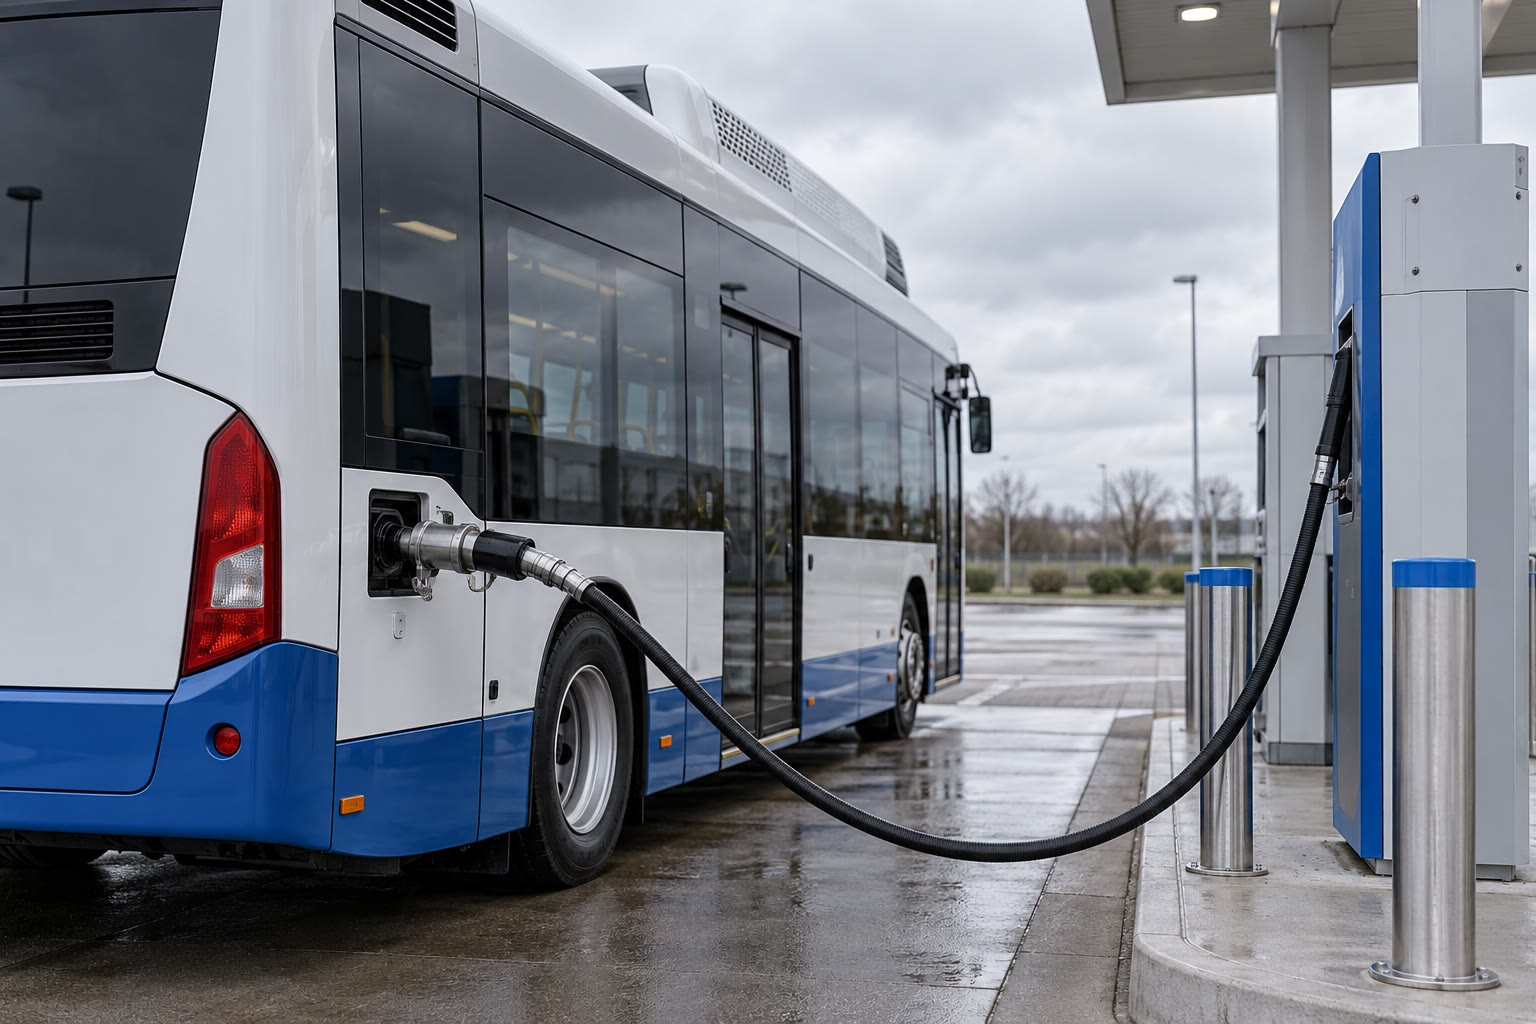
\includegraphics[width=0.5\linewidth]{images/book1/ai/g11-hydrogen-bus.jpg}

{\small हाइड्रोजन स्टेशन पर एक बस: उसका \omterm{def:g4:what-a-fire-needs:fuel}{ईंधन} केवल पानी छोड़ता है।}
\end{omfigure}

\begin{safety}{\ghs[0.82cm]{GHS02}\ghs[0.82cm]{GHS07}}
% ledger: ghs:ethanol
एथेनॉल अत्यंत ज्वलनशील है और आँखों में जलन पैदा करता है। स्पिरिट लैंप
किसी भी लौ से दूर भरा जाता है, गरम रहते कभी दोबारा नहीं भरा जाता, और
शिक्षक इसे ऊष्मारोधी चटाई पर इस्तेमाल करते हैं।
\end{safety}

\section{अभ्यास}


\begin{exercise}[$\star$]\label{exo:g11:reaction-energy:1}
\omterm{def:g11:reaction-energy:exothermic}{ऊष्माक्षेपी} या \omterm{def:g11:reaction-energy:exothermic}{ऊष्माशोषी}: लकड़ी का \omterm{def:g4:what-a-fire-needs:burning}{जलना}; बर्फ़ का पिघलना; शीत पैक का
दबाया जाना; हाथ गरम करने वाली थैली का गरम होना; हरी पत्ती का धूप में
शर्करा बनाना?
\end{exercise}

\begin{exercise}[$\star$]\label{exo:g11:reaction-energy:2}
% ledger: dch:CH4
मेथेन के \qty{3.0}{mol} का \omterm{def:g8:combustion-and-fuels:complete}{पूर्ण दहन} कितनी ऊर्जा
मुक्त करता है?
\end{exercise}

\begin{exercise}[$\star$]\label{exo:g11:reaction-energy:3}
\omterm{def:g11:reaction-energy:exothermic}{ऊष्माक्षेपी} अभिक्रिया के ऊर्जा आरेख पर किसमें अधिक
ऊर्जा है, \omterm{def:g7:chemical-reactions:reactant}{अभिकारकों} में या उत्पादों में? अंतर कहाँ जाता है?
\end{exercise}

\begin{exercise}[$\star$]\label{exo:g11:reaction-energy:4}
% ledger: dch:C2H5OH
\qty{100}{g} एथेनॉल का \omterm{def:g8:combustion-and-fuels:complete}{पूर्ण दहन} कितनी ऊर्जा
मुक्त करता है?
\end{exercise}

\begin{exercise}[$\star$]\label{exo:g11:reaction-energy:5}
\omterm{def:g11:reaction-energy:bond-energy}{आबंध ऊर्जा} क्या है? आबंध तोड़ने में हमेशा ऊर्जा क्यों लगती है?
\end{exercise}

\begin{exercise}[$\star\star$]\label{exo:g11:reaction-energy:6}
\omterm{def:g11:reaction-energy:bond-energy}{आबंध ऊर्जाओं} से अभिक्रिया
\ce{2H2 + O2 -> 2H2O} की ऊर्जा का अनुमान लगाइए, सभी गैसें। क्या यह \omterm{def:g11:reaction-energy:exothermic}{ऊष्माक्षेपी} है?
\end{exercise}

\begin{exercise}[$\star\star$]\label{exo:g11:reaction-energy:7}
\omterm{def:g11:reaction-energy:bond-energy}{आबंध ऊर्जाओं} से एथेनॉल के \omterm{def:g4:what-a-fire-needs:burning}{दहन}, \ce{C2H5OH + 3O2 ->
2CO2 + 3H2O}, की ऊर्जा का अनुमान लगाइए (पहले एथेनॉल की \omterm{def:g10:lewis-and-shape:lewis-structure}{लुइस संरचना}
बनाइए), और मापे गए \qty{1367.6}{kJ/mol} से तुलना कीजिए।
\end{exercise}

\begin{exercise}[$\star\star$]\label{exo:g11:reaction-energy:8}
% ledger: dch:C3H8, dch:CH4
प्रोपेन (\qty{2219.2}{kJ/mol}) और मेथेन के प्रति किलोग्राम मुक्त ऊर्जा
निकालिए। दंड आलेख से तुलना कीजिए।
\end{exercise}

\begin{exercise}[$\star\star$]\label{exo:g11:reaction-energy:9}
% ledger: cp:water, dch:CH4
एक गैस चूल्हा \qty{1.50}{L} पानी (\qty{1500}{g}) को
\qty{15}{\celsius} से \qty{100}{\celsius} तक गरम करता है। पानी कितनी ऊर्जा
ग्रहण करता है? यदि सारी ऊर्जा पानी तक पहुँचे तो मेथेन का कितना द्रव्यमान
\omterm{def:g4:what-a-fire-needs:burning}{जलता} है? यदि उसका केवल आधा ही पहुँचे तो?
\end{exercise}

\begin{exercise}[$\star\star$]\label{exo:g11:reaction-energy:10}
दंड आलेख की मदद से \omterm{def:g4:what-a-fire-needs:fuel}{ईंधनों} को प्रति किलोग्राम ऊर्जा के क्रम में रखिए। हाइड्रोजन
का कितना द्रव्यमान \qty{1.0}{kg} ऑक्टेन जितनी ऊर्जा देता है?
\end{exercise}

\begin{exercise}[$\star\star$]\label{exo:g11:reaction-energy:11}
\ce{N2 + 3H2 -> 2NH3} की ऊर्जा का अनुमान लगाइए, सभी गैसें। \omterm{def:g11:reaction-energy:exothermic}{ऊष्माक्षेपी} या
\omterm{def:g11:reaction-energy:exothermic}{ऊष्माशोषी}?
\end{exercise}

\begin{exercise}[$\star\star\star$]\label{exo:g11:reaction-energy:12}
% ledger: cp:water, dch:C2H5OH
स्पिरिट लैंप वाले एक प्रयोग में \qty{1.20}{g} एथेनॉल \omterm{def:g4:what-a-fire-needs:burning}{जलने} के दौरान \qty{250}{g} पानी
\qty{20}{\celsius} गरम होता है। पानी द्वारा ग्रहण की गई
ऊर्जा, एथेनॉल द्वारा मुक्त की जा सकने वाली ऊर्जा, और
तापन की दक्षता निकालिए। हानियों के तीन कारण बताइए।
\end{exercise}

\begin{exercise}[$\star\star\star$]\label{exo:g11:reaction-energy:13}
% ledger: dfh:C8H18, dfh:CO2, dfh:H2O-l, dch:C3H8
ऑक्टेन \qty{5470}{kJ/mol} और प्रोपेन \qty{2219.2}{kJ/mol} मुक्त करते हैं।
उनके \omterm{def:g4:what-a-fire-needs:burning}{दहन} समीकरण लिखिए और हर एक द्वारा प्रति मेगाजूल मुक्त कार्बन डाइऑक्साइड
का द्रव्यमान निकालिए। मेथेन, \qty{49.4}{g}, से तुलना कीजिए।
\end{exercise}

\begin{exercise}[$\star\star\star$]\label{exo:g11:reaction-energy:14}
मेथेन और एथेनॉल दोनों के लिए आबंध-ऊर्जा अनुमान मापी गई
मुक्त ऊर्जा से कम है। कारण बताइए, और समझाइए कि
अनुमान फिर भी उपयोगी क्यों है।
\end{exercise}

\begin{exercise}[$\star\star\star$]\label{exo:g11:reaction-energy:15}
\ce{2H2O -> 2H2 + O2} की ऊर्जा का अनुमान लगाइए, सभी गैसें। पानी से हाइड्रोजन
बनाने के लिए ऊर्जा (उदाहरण के लिए बिजली के रूप में) क्यों देनी पड़ती है?
समझाइए कि हाइड्रोजन को ऊर्जा का स्रोत होने के बजाय ऊर्जा \emph{संचित}
करने का एक साधन क्यों कहा जाता है।
\end{exercise}

\section{समस्या: शहर की बस के लिए कौन-सा ईंधन?}

\begin{problem}[{सप्ताहांत समस्या --- मेथेन, एथेनॉल, ऑक्टेन या हाइड्रोजन:
प्रति किलोग्राम सबसे अधिक ऊर्जा कौन देता है, और प्रति मेगाजूल
कितनी कार्बन डाइऑक्साइड?}]
\label{pb:g11:reaction-energy:1}
% ledger: dch:CH4, dch:C2H5OH, dfh:C8H18, dfh:CO2, dfh:H2O-l, be:C-H, be:OO-double, be:CO-double, be:O-H
एक शहर अपनी बसों के लिए चार \omterm{def:g4:what-a-fire-needs:fuel}{ईंधनों} की तुलना करता है: मेथेन (प्राकृतिक गैस), एथेनॉल,
ऑक्टेन (पेट्रोल के लिए) और हाइड्रोजन। एक \omterm{def:g10:the-mole:amount}{मोल} के \omterm{def:g8:combustion-and-fuels:complete}{पूर्ण दहन} द्वारा मुक्त
ऊर्जाएँ हैं: मेथेन \qty{890.7}{kJ}, एथेनॉल
\qty{1367.6}{kJ}, ऑक्टेन \qty{5470}{kJ}, हाइड्रोजन \qty{285.8}{kJ}, बनने वाला
पानी द्रव मानकर।

\medskip
\noindent\textbf{भाग I --- \omterm{def:g4:what-a-fire-needs:burning}{दहन} समीकरण।}
\begin{enumerate}
  \item मेथेन के \omterm{def:g8:combustion-and-fuels:complete}{पूर्ण दहन} का समीकरण लिखिए।
  \item एथेनॉल, \ce{C2H6O}, का।
  \item ऑक्टेन, \ce{C8H18}, का।
  \item हाइड्रोजन का।
  \item कौन-सा \omterm{def:g4:what-a-fire-needs:fuel}{ईंधन} कोई कार्बन डाइऑक्साइड मुक्त नहीं करता?
\end{enumerate}

\medskip
\noindent\textbf{भाग II --- प्रति किलोग्राम ऊर्जा।}
\begin{enumerate}[resume]
  \item चारों \omterm{def:g4:what-a-fire-needs:fuel}{ईंधनों} के \omterm{def:g10:the-mole:molar-mass}{मोलर द्रव्यमान} निकालिए।
  \item हर एक के लिए प्रति किलोग्राम मुक्त ऊर्जा
        \si{MJ/kg} में निकालिए।
  \item \omterm{def:g4:what-a-fire-needs:fuel}{ईंधनों} को क्रम में रखिए।
  \item हाइड्रोजन बहुत आगे है। फिर भी उसे बस में ले जाना कठिन क्यों
        है? (कमरे के ताप पर उसकी अवस्था के बारे में सोचिए।)
\end{enumerate}

\medskip
\noindent\textbf{भाग III --- \omterm{def:g11:reaction-energy:bond-energy}{आबंध ऊर्जाओं} से अनुमान।}
\begin{enumerate}[resume]
  \item मेथेन के \omterm{def:g4:what-a-fire-needs:burning}{दहन} में शामिल \omterm{def:g7:atoms-and-molecules:molecule}{अणुओं} की \omterm{def:g10:lewis-and-shape:lewis-structure}{लुइस संरचनाएँ} बनाइए,
        और टूटे और बने आबंध गिनिए।
  \item आबंध तोड़ने के लिए आवश्यक ऊर्जा निकालिए।
  \item नए आबंध बनने से मुक्त ऊर्जा निकालिए।
  \item $E_r$ का अनुमान निकालिए, और मापे गए मान से
        तुलना कीजिए: सापेक्ष अंतर?
  \item अंतर के दो कारण बताइए।
\end{enumerate}

\medskip
\noindent\textbf{भाग IV --- प्रति मेगाजूल कार्बन डाइऑक्साइड।}
\begin{enumerate}[resume]
  \item \qty{1}{MJ} मुक्त करने के लिए मेथेन की कितनी मात्रा जलनी चाहिए?
  \item वह कार्बन डाइऑक्साइड का कितना द्रव्यमान मुक्त करती है?
  \item एथेनॉल और ऑक्टेन के लिए यही प्रश्न।
  \item समान ऊर्जा के लिए कौन-सा कार्बन \omterm{def:g4:what-a-fire-needs:fuel}{ईंधन} सबसे कम कार्बन डाइऑक्साइड
        मुक्त करता है? क्यों (C और H \omterm{def:g7:atoms-and-molecules:atom}{परमाणुओं} की संख्याओं की तुलना कीजिए)?
  \item \omterm{def:g4:what-a-fire-needs:burning}{जलने} पर हाइड्रोजन कुछ भी मुक्त नहीं करती। जलवायु के लिए उसका
        वास्तविक लाभ किस पर निर्भर करता है?
  \item अंतिम उत्तर बताइए: मेथेन प्रति मेगाजूल कार्बन डाइऑक्साइड का कितना
        द्रव्यमान मुक्त करती है?
\end{enumerate}
\end{problem}
